% !TeX root = ../main.tex

\chapter{Implementation}
\label{ch:implementation}
For the evaluation of various image recognition algorithms on different kinds of food datasets a program called \acrfull{tfc} was implemented. It is able to calculate several performance measurements, load and preprocess image datasets, use these datasets to train image classifiers from different libraries and optimize classifier parameters.  

Section \ref{sec:infrastructure} gives general information about the infrastructure of the program and section \ref{sec:modules} describes the modules in detail.


\section{Infrastructure}
\label{sec:infrastructure}

	\subsection{Architecture}
	\begin{figure}
		\centering
		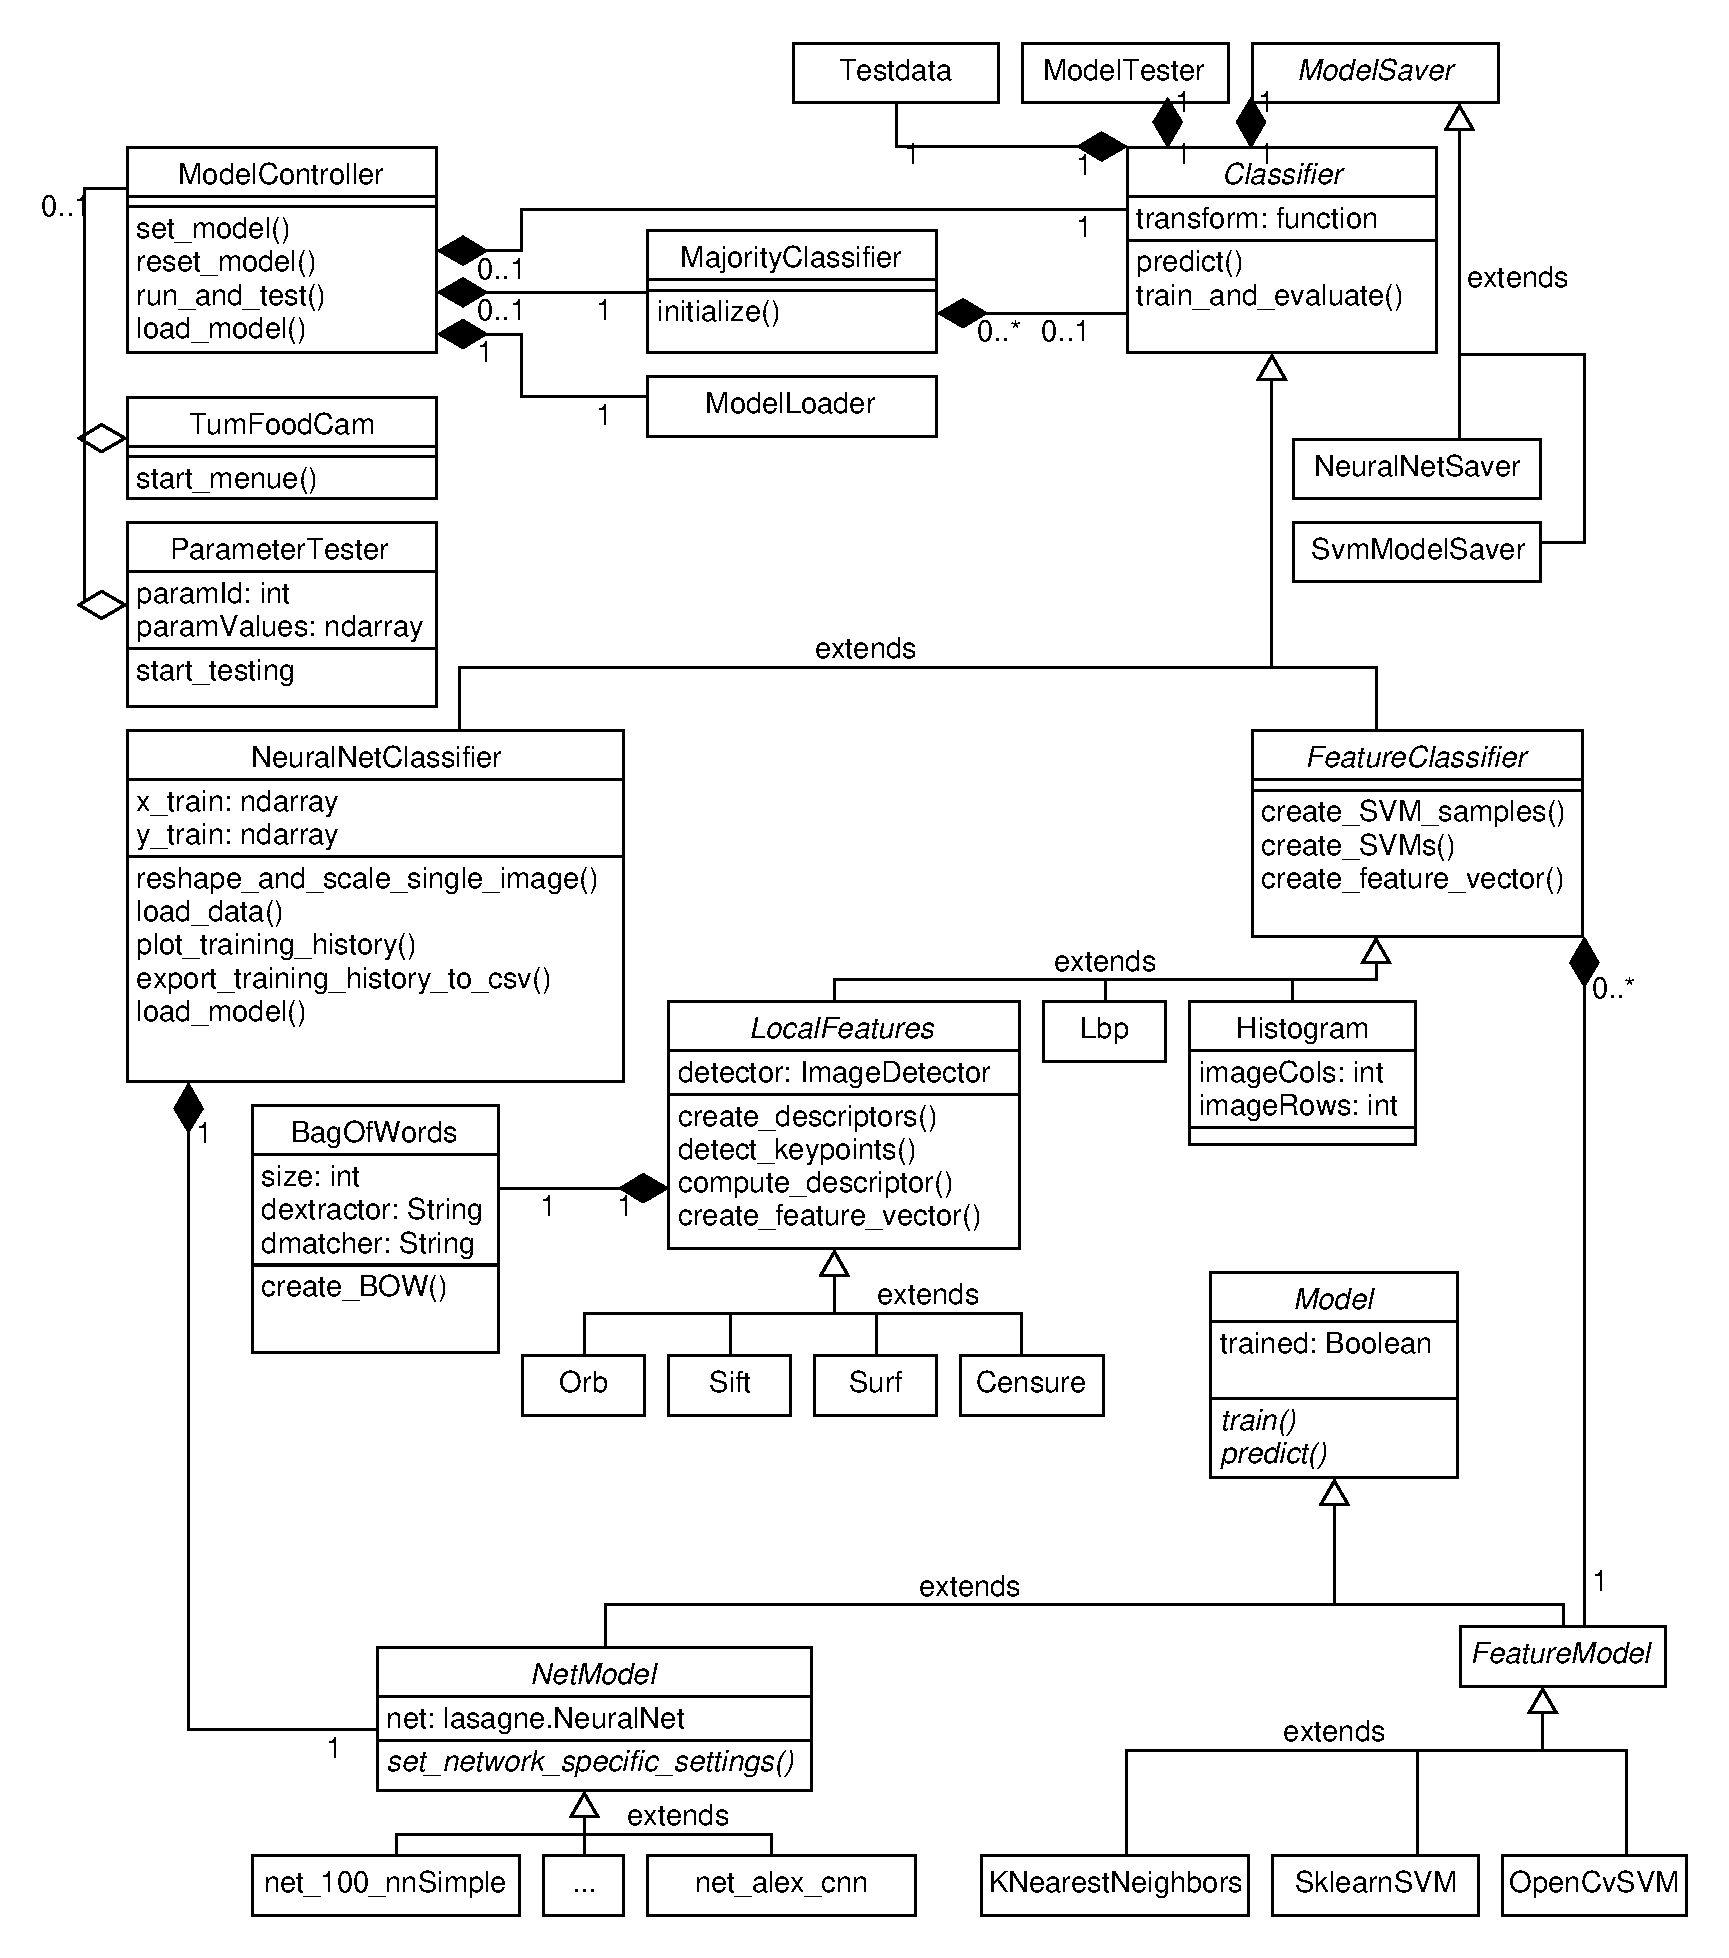
\includegraphics[width=\linewidth]{figures/implementation_classDiagram}
		
		\caption{Reduced class diagram of TumFoodCam architecture.}
		\label{fig:classDiagram}
	\end{figure}
	Figure \ref{fig:classDiagram} describes the architecture of the most important classes. The class diagram does not show all classes, methods and attributes but only the general relationship and interaction between the classes. This was necessary because the scope of the program is quite big and including all data would not have helped to understand the overall view.
	
	All classifiers in the "TUM Food Cam" application are controlled by the \textit{ModelController} Singleton. Both the main class \textit{TumFoodCam} as well as the class \textit{ParameterTester} use the controller to create and load classifers. The \textit{ModelController} instantiates exactly one \textit{Classifier} object which can either be a \textit{NeuralNetClassifier} or a \textit{FeatureClassifier}. \textit{Classifier} is an abstaract\footnote{since there are no abstract classes or interfaces in python, an "abstract" class is implemented by raising a \textit{NotImplementedError} in each method body.} class that provides access to \textit{ModelSaver},  \textit{Testdata} and the \textit{ModelTester} class.
	
	\textit{NeuralNetClassifier} contains one \textit{NetModel} which is an abstract wrapper for a concrete neural net architecture like \textit{net\_100\_nnSimple} and extends the abstract \textit{Model} class. \textit{FeatureClassifier}, the other class that extends \textit{Classifier}, provides methods for the creation and management of \glspl{svm} or k-nearest-neighbors. \textit{Histogram} and \textit{Lbp} derive directly from \textit{FeatureClassifier} since they both calculate a global feature vector that can be used directly for \gls{svm} training. The other classifiers extend \textit{LocalFeatures} which derives from \textit{FeatureClassifier}. \textit{LocalFeatures} controls the creation of keypoints, descriptors as well as training and use of a \gls{bow}. The classification of the images is done by one or multiple instances of \textit{FeatureModel}.
	
	Almost all parameters for methods and general application behavior are globally defined in the \textit{Settings} module. Settings can be loaded and saved by the \textit{SettingsService} {(not part of figure \ref{fig:classDiagram})}.
	
	\subsection{Patterns}
	
		\subsubsection*{Strategy Pattern}
		The application uses several different libraries for classification and feature extraction. To unify the general process of learning, all classifiers are abstracted by the \textit{Classifier} class. It acts as an interface and mainly declares two methods to train and predict images. Subclasses will implement those methods so that the \textit{ModelController} does not need to know the difference of training a neural net or a \gls{svm} feature classifier which makes it possible to chose a classifier at runtime and add new classifiers easily. This pattern is called "Strategy pattern".
	
		\subsubsection*{Template Pattern}
		The "Template pattern" is almost the same as the strategy pattern but is applied on the \textit{FeatureClassifier} level. \textit{FeatureClassifier} is an abstract class and provides methods for \gls{svm} creation. It acts as a template for any feature classifier that relies on \glspl{svm}. 
		
		\subsubsection*{Facade Pattern}
		This pattern is applied at the last layer where the actual \gls{api} is accessed. There is no common naming convention between different \glspl{api} so although \verb|censure.detect(image)| and  \verb|sift.detect(image)| might have the same syntax, they work differently because OpenCV returns the keypoints and skimage does not. Classes like \textit{Sift} or \textit{Censure} therefore have to act as a wrapper or facade for the actual \gls{api} calls and unify them for their super-classes.
	
		
	
	
	
	\subsection{Libraries}
		
		\subsubsection*{OpenCV}
		\label{subsubsec:openCV}
		OpenCV which stands for "Open Source Computer Vision" is a cross platform framework with over 2,500 optimized algorithms \cite{bradski2000opencv, openCVWebsite}. OpenCV is written in C++ and includes a wide variety of computer vision algorithms, image recognition toolkits and a machine learning library and is the de facto standard for computer vision. OpenCV is licensed under BSD which makes it free for academic and commercial use\footnote{SIFT and SURF are patented \cite{Lowe2004a} \cite{Funayama2012} and should not be used in commercial applications.}. OpenCV is the most important library in \gls{tfc} because it handles most image file \gls{io}, transformations and classification.
		
		\subsubsection*{Scikit-learn}
		Scikit-learn or sklearn is an open source machine learning library for python \cite{Pedregosa2011}. Scikit-learn is used because its LibSVM implementation is much more open and allows more kernels than OpenCV does.
		
		\subsubsection*{Scikit-image}
		Scikit-image is a library with many image processing and computer vision algorithms \cite{scikit-image}. It provides keypoint detectors and descriptors like \gls{hog} or \gls{censure} that OpenCV does not include.
		
		\subsubsection*{Lasagne and Nolearn}
		Lasagne is a library that is used to build and fit neural networks in Theano \cite{Dieleman2015}. Lasagne was selected as the library for all neural networks because it is based on theano, a commonly used numerical computation library which supports \gls{cuda} for efficient execution on \glspl{gpu}. Lasagne adds a layer of abstraction to theano which makes it easier to create and train neural networks because it specifically sets the focus on an easy to learn syntax that is compatible to sklearn.
		
		Lasagne is further refined by nolearn which makes the process of neural network architecture creation even more easier to read and provides additional useful methods for the training and visualization process like layer activations. All neural networks in this application are nolearn-lasagne-theano nets. 
		

\section{Modules}
\label{sec:modules}

	\subsection{Input / Output}
	The \textit{data\_io} package contains modules focused on the input and output of data.
	\begin{figure}
		\centering
		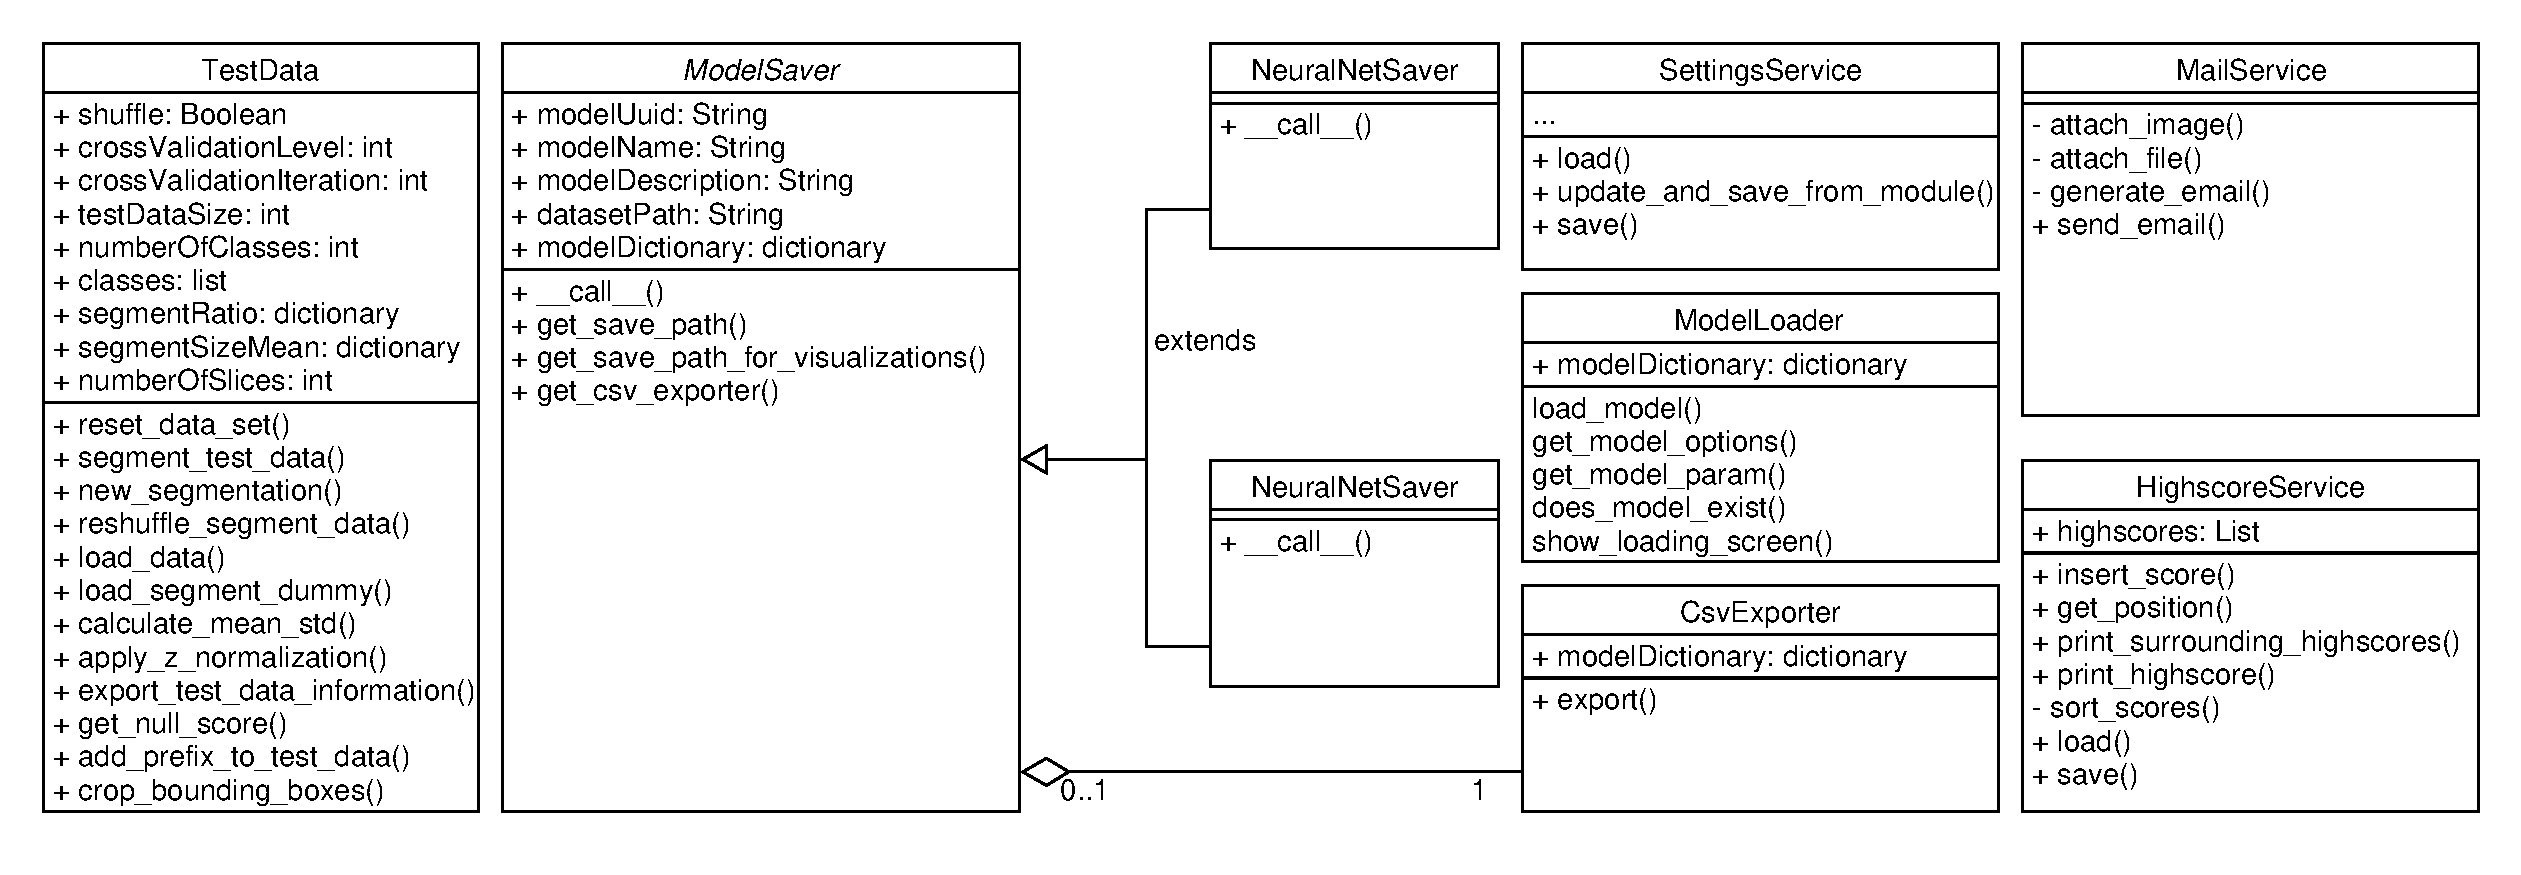
\includegraphics[width=\linewidth]{figures/implementation_dataIO}		
		\caption{Class diagram of data\_io package.}
		\label{fig:dataIO}
	\end{figure}
	
		\subsubsection*{Test Data Module}
		This module manages and loads data from different image datasets. It builds a class directory by iterating over the folders in the dataset root path. Depending on \verb|crossValidationLevel| which is the $k$ in $k$-fold cross validation and \verb|segmentRatio| it slices the data into $k$ parts. After each cross validation iteration \verb|new_segmentation()| should be called which shifts the segments for a new validation. After the last iteration it returns \verb|False|. 
		
		\verb|load_data()| is the method which iterates over the actual images. It can be called with different parameters to restrict certain classes, the number of images per class, or apply different transformation, data preprocessing and size specifications.
		
		\subsubsection*{ModelIO Service}
		\textit{model\_io} is a module which contains classes for saving and loading of models as well as a class to export data to \gls{csv} files. \textit{NeuralNetSaver} and \textit{SvmModelSaver} both derive from \textit{ModelSaver}. \textit{ModelSaver} manages the save directory of the model by giving each model a unique id which is saved in the \verb|modelDictionary|.
		
		\subsubsection*{Settings Service}
		The class \textit{SettingsService} uses the global settings variables in the module \textit{settings} to store and restore the settings.
			
	\subsection{Neural network modules}
			
		\subsubsection*{Neural networks}
		There are several modules in the "deep" package which is a sub-package of "classification". \textit{neural\_net} includes the \textit{NeuralNetClassifier} which is the central controller class for every neural network. It instantiates a \textit{NetModel}, loads dummy data in case the dataset will be augmented or loaded lazily and provides data logging methods.
		
		Classes that extend \textit{NetModel} are the wrappers for the actual neural net \gls{api}. They each instantiate a specific net architecture. For better evaluation and training performance these classes are able to make use of the modules \textit{batch\_iterators}, \textit{learning\_functions} and \textit{training\_history}.
		
		The module \textit{batch\_iterators} manages the loading of image batches for each iteration. It contains the classes:
		\begin{itemize}
			\item\textit{LazyBatchIterator} which only loads image batches when they are needed. Without it the whole dataset would have to be loaded into memory prior to the training.
			\item\textit{AugmentingBatchIterator} which augments images. The process is detailed in section \ref{subsec:dataAugmentation}.
			\item\textit{AugmentingLazyBatchIterator} is a combination of both batch iterators.
		\end{itemize}
	
		\textit{learning\_functions} contains the classes \textit{AdjustVariable} and \textit{EarlyStopping}. Both are explained in section \ref{subsec:setupNN}.
		
		\textit{training\_history} provides methods for logging and plotting of the model fitting.
	
	\subsection{Testing}
	
	\begin{figure}
		\centering
		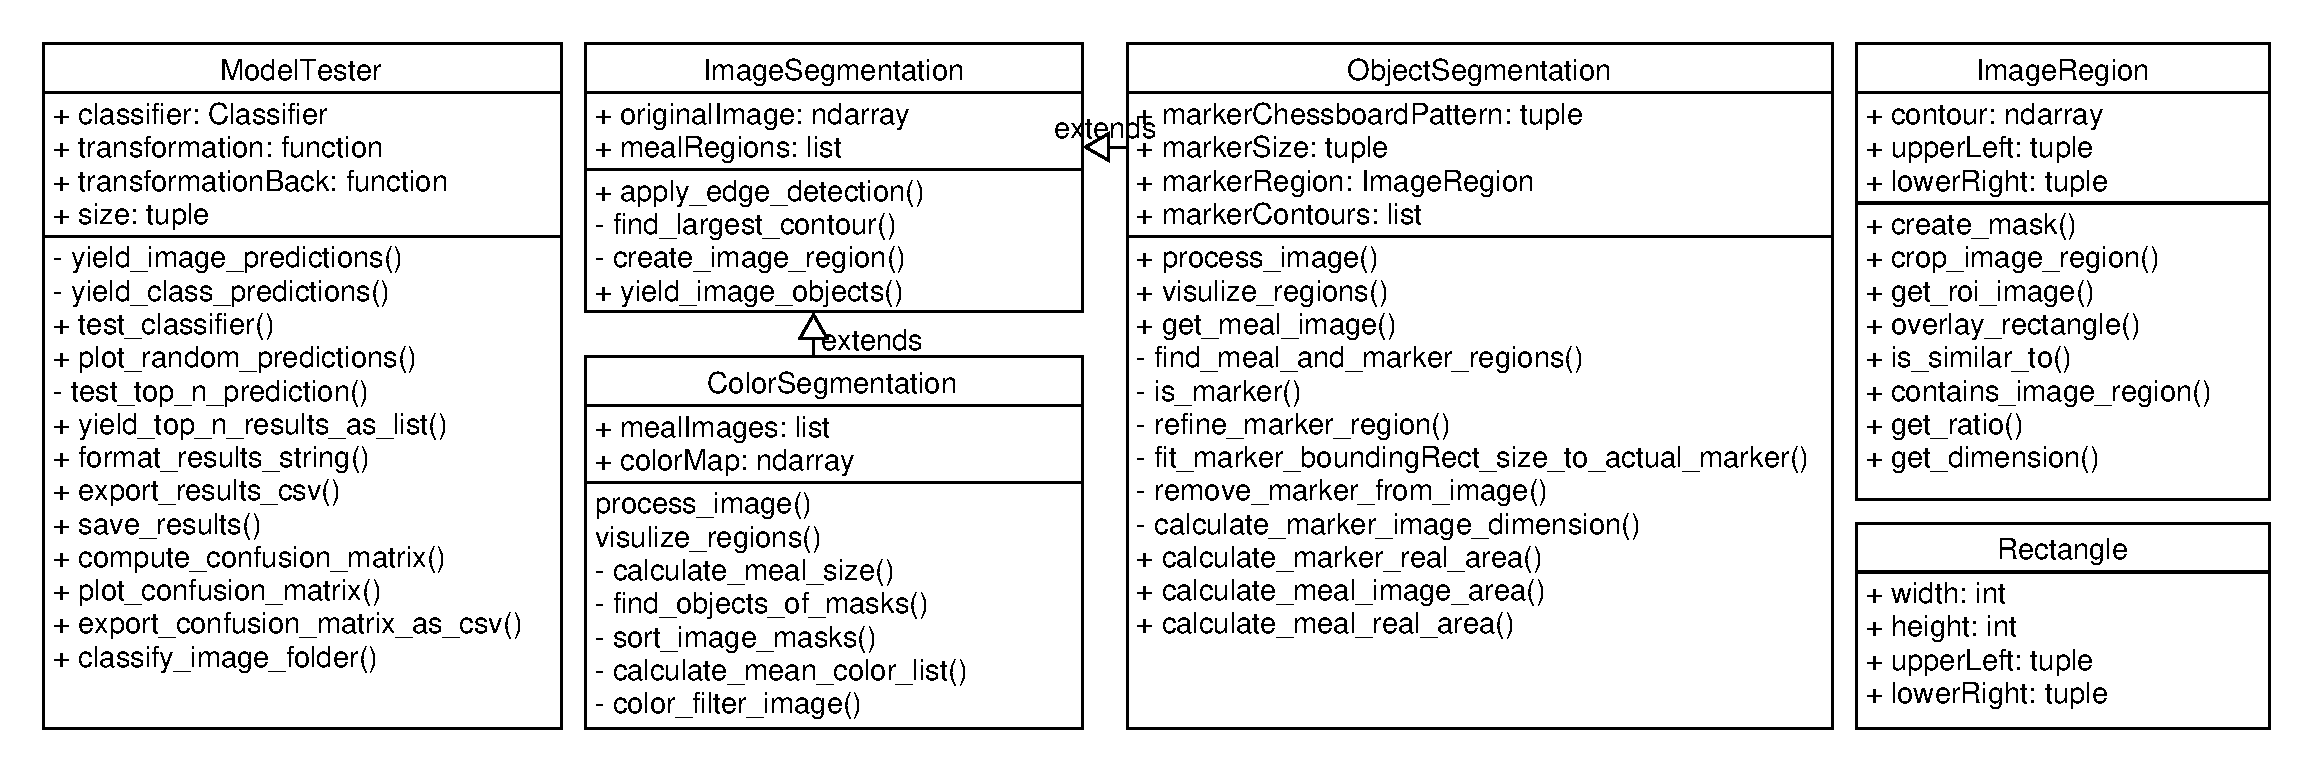
\includegraphics[width=\linewidth]{figures/implementation_misc_segmentation}
		
		\caption{Class diagram of ModelTester and classes from the segmentation package.}
		\label{fig:testerSegmentation}
	\end{figure}
		\subsubsection*{Model Tester}	
		The task of \textit{ModelTester} is the evaluation of models. Calling \verb|test_classifier()| on a test data segment will test the classifier by comparing the predicted class to the actual class. For each class as well as for the whole segment the accuracy, recall and precision are calculated and exported. The class does also plot a confusion matrix and a prediction of random images visualization. 
		
		\subsubsection*{Parameter Tester}
		\textit{ParameterTester} is part of the \textit{model\_controller} module. Given a classifier, and a \textit{Testsuite} with a list of parameters and corresponding parameter values it will test each parameter value on the classifier and plot and export the results.	
	
	\subsection{Image Segmentation}
	\textit{image\_segmentation} contains 3 image segmentation classes for segmentation, meal area size estimation and meal part size estimation.
	\begin{itemize}
		\item\textit{ImageSegmentation} is the super class for \textit{ObjectSegmentation} and \textit{ColorSegmentation}. It applies canny edge detection and image dilation and provides a method which iterates over found image objects detected by the OpenCV \verb|findContours()| algorithm.
		\item\textit{ObjectSegmentation} searches for the meal and a marker and approximates, based on the marker, the area of the meal.
		\item\textit{ColorSegmentation} further analyzes the meal region for different meal parts by applying selective color filtering. For each meal region the size is approximated.
	\end{itemize}
	
	\subsection{Helper Functions}
	The \textit{utils} contains over 60 functions used in all program parts from image transformations over console menus and output.

